\chapter{如何降低软件开发质量成本} % Introduction chapter suppressed from the table of contents

软件开发不同于工业生产,因都是人的行为,依赖团队成员自己收集。(工业生产依赖自动化机器,容易得到数据。)

\hypertarget{ux6570ux636eux6536ux96c6}{%
\subsection{数据收集}\label{ux6570ux636eux6536ux96c6}}

``如何才能收集到开发质量相关数据,来分析根因,制定纠正改进措施?
因为没有度量,便无法谈改进。''这是很多研发经理想解决的问题。\\
收集软件开发数据有各种困难,如果没有收集到可信的数据,便无从分析与改进。\\
是否可以依赖加强组织级度量与监控?
我们先看看一家过万人,主要提供金融软件产品,公司遇到的困难,公司一直都很强调量化管理,收集各种项目的系数、度量并分析。\\

\hypertarget{ux81eaux52a8ux5316ux7edfux8ba1ux5206ux6790}{%
\subsection{自动化统计分析}\label{ux81eaux52a8ux5316ux7edfux8ba1ux5206ux6790}}

质量部经理:我们每次都跑全量,公司引入低码平台,更多的是在需求设计阶段做好质量保证,
所以我们很注重量化质量管理,能否通过自动化来统计分析,
如何通过量化或工具方式实现自动评审。

我:为什么要自动化?

经理:从去年开始我们搞度量分析, 发现员工就会造数据, 结果导致失真,
度量哪里就造哪里,
所以还是想通过工具代替人工方式,除了能提升效率,也能帮助判断数据是否合理。\\
现在我们的主管很反感度量,一度量就有人造数据。

我:度量本来是件好事。 经理:是的,就是大家知道算法原理就开始造假。
因为我们搞了红黑榜,
但很多人头脑都很聪明,会想办法,但用于不合适的地方。

我们有很多数据统计分析,比如看测试用例与需求的比例。
其实客户发现的缺陷比例也降低了,但因为我们这行对质量特别注重,产品经过多年的逐步演化,过程很复杂,导致软件缺陷的修复很耗时,客户不太满意。
而且公司要求交付的频率要比以前高了很多,我们团队做这些分析都忙不过来,所以需要员工设自动化工具等加快速度才可以。\\
让我给你看看我们大数据分析。

我:等等,但我们首要解决如何能收集到真正的数据,不然数据分析没有意义。

经理:好的,有什么建议?

我:还记得我们上次交流,要让团队自主,不能单靠标准过程并用指标监控执行情况。

%\href{文件:Diagram_2.0.png}{500px}

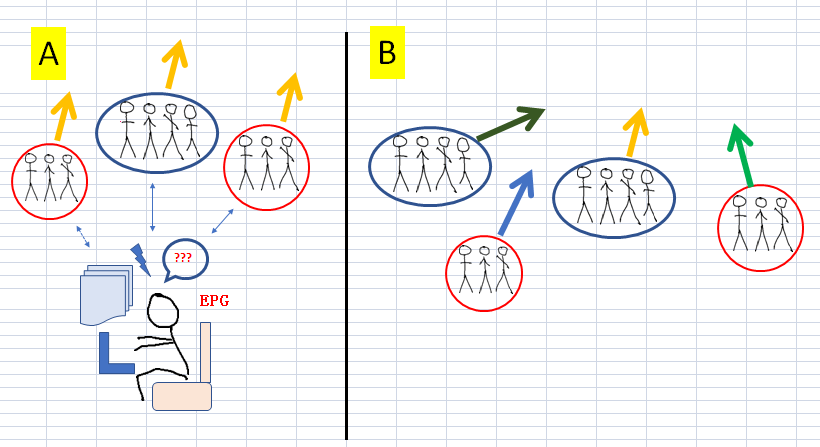
\includegraphics[width=6cm]{Diagram_20.png}

我:请问你们是采用左面还是右面的方法做过程改进?\\
经理:好像我们现在度量分析是采用你图里左面的方法。

我:是的。总体分析还有另一不足:各个项目特性不一样,你们现在几十个项目总体趋势分析,
很可能找不对根因,因每个项目的问题(根本原因)很可能不同。
比如,同样是一个测试用例比例数,你的范围就很宽,从最低的0.3到最高的超过200。但你们取平均值5.1
来做分析。

收集数据也是问题,因为收集数据是挺花精力的工作。

经理:完全同意。

我:但正因为不同项目有各种特性,要对收集到的数据做分析也很耗时。
这些辛辛苦苦做出来的分析报告其实不仅仅是给高层(或者项目经理),
使每一个团队成员都看到才有意义
。(度量分析要反馈回数据提供者,他们才有动力继续收集数据)要把那些分析好的报告再跟每一个团队成员解释要花多大精力?

\textbf{度量的主要目的是从数据分析找出根因做改进而不是仅仅为了监控}

%\href{文件:Ma4CarScreenshot_2021-12-27_205004.png}{400px}

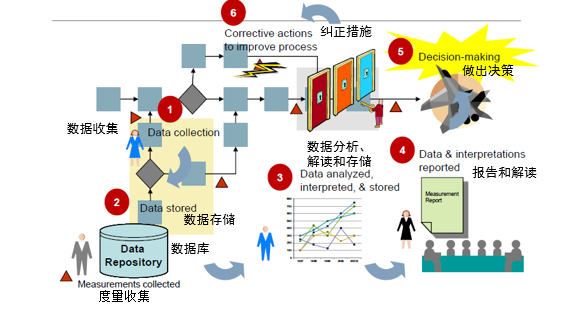
\includegraphics[width=6cm]{Ma4CarScreenshot_2021-12-27_205004.png}

如果把数据分析下放到团队自己搞,便灵活多了;也正因为他们有参与收集和分析讨论,
你们也可以节省很多沟通的成本。

所以你们领导应该定位自己是内部老师,辅导团队怎么做好数据分析,效果会更好。

经理:团队自己讨论便可以得到改进吗?不需要我们领导?\\
我:
如果团队有能力,就应该放手让他们自己收集数据、利用数据进行分析并做出改进。你们应把自己重新定位为团队的教练,去辅导他们如何收集与分析数据。千万不要以为这项工作会比以前自己做分析更轻松,其实你们需要更熟悉整个过程,才能真正辅导好团队。但因为你们之前积累了经验,所以辅导团队应该不会太难。更大的挑战反而是要让管理层了解并赞同,敏捷开发需要团队自主的思路。

\hypertarget{ux6570ux636eux6536ux96c6ux9891ux7387}{%
\subsection{数据收集频率}\label{ux6570ux636eux6536ux96c6ux9891ux7387}}

几个月后,质量经理问:请问老师有没有写过关于客户满意度与产品研发/质量/过程改进之间的关系的文章?我想从研发改进或质量改进的角度,正向推导出如何帮助提升客户满意度的方法。

\begin{description}
\tightlist
\item[]
(公司一直很注重每年的客户满意度调查,高层也会参考满意度调查结果,作为
KPI系数之 一,确定绩效,并决策公司资源的投放等。)\\
\end{description}

我:我没有写过你说的这类分析文章,但有写过客户的案例分享:某香港公司,他们在广州有开发中心专门为香港的客户做软件维护工作,他们的项目采用
SCRUM
敏捷开发,每两周一个冲刺,他们每次做完迭代后,都会要求客户填写满意度调查表,然后做数据分析。(这分享文章的部分内容,详见附录B:``分析迭代客户满意度调查数据'')\\
经理:我刚才看了你发的案例分享,挺好的,但我想要的不是通过分析每一次迭代的客户满意度,让团队做过程改进,我想更宏观一些。每年,我们公司有独立部门做客户满意度调查,已经持续了十年,高层会根据调查的结果判断是否继续向事业部投放资源,也会影响到员工绩效等等,所以其他部门都很关注。但后面越来越发现那些数据的作用不大,因为各事业部都清楚,客户满意度调查的分数很重要,高层也关注,所以都会在调查之前拜访客户,做好准备,确保结果不会太差。\\
我:你们做了这么多年,应该最清楚自己的问题所在,你觉得现在的做法有什么不足?\\
经理:我们的客户满意度调查是每年随机抽样一些客户来做,因为是抽样,又是在每年年底才做,有些时候可能项目在上半年的四五月已经结束了。到年底时,客户对很多几个月前的情况都忘记了。\\
我:是的,为什么不在项目发布后立马就做?\\
经理:这项工作是由独立部门去做,因工作量比较大,每年都是独立策划安排的。其实我们也有在项目发布后就做的调查,不过时间跨度没有年度这么宽。只是一些简单的高中低打分,由一线人员直接去做。\\
我:为什么不能安排你们的客户满意度调查也是在项目的结束时间去开展,这样不就更及时吗?\\
经理:主要是他们的人力有限,资源有限。\\
我:这个不太说得通,我没有说你们每次发布后都要做调查,这会增加工作量,但你们还是可以随机抽样调查,这样及时性就好多了,不会等到几个月后才调查。你们为什么只在每年年底做调查并更新标杆?\\
经理:还有另一个原因,高管很注意客户满意度调查的结果,以此来判断部门的绩效和对事业部的资源投放,所以调查需要与公司年底的预算同步。\\
我:标杆(基线)的更新不应每年只更新一次,而是实时变化的,如果有显著的变化就更新。还有一个问题,你刚才说因为客户满意度调查的结果会被公司高管用来判断部门的绩效和对事业部的资源投放,所以业务部门肯定会非常关注,并想尽办法得到好的结果,比如预先拜访等等。其实这个不但污染了数据本身的准确性,也影响了数据的可信度,让数据变得不客观。\\
经理:好的,我会根据你的意见,在明天讨论如何改革客户满意度调查时,提出建议。\\


\hypertarget{ux54eaux91ccux6700ux8017ux5de5ux4f5cux91cf}{%
\subsection{哪里最耗工作量}\label{ux54eaux91ccux6700ux8017ux5de5ux4f5cux91cf}}

软件开发特点,超过95\%的成本都是人力成本。按二八原则,应先识别最耗工作量的地方?

首先利用二八原则识别出哪类问题的影响最大。在软件开发中,如想提升团队生产率(降低工作量),应先探索哪类工作最耗费工时。

\framebox{%
\begin{minipage}[t]{0.97\columnwidth}\raggedright
\textbf{请你把过去一年的软件开发项目,按不同工种占项目总工作量的比例,从最多到最少排个序?}

\begin{enumerate}
\tightlist
\item
  编码与代码设计
\item
  交付后的所有工作,包括维护、更新与缺陷修正
\item
  交付前的评审,静态扫描,测试与缺陷修正
\item
  项目管理与监控
\end{enumerate}\strut
\end{minipage}}

可以参考本章附件中的“开发项目工作量(成本)分布”,看你的选择与典型分布相差多远。

软件开发项目最大的工作量通常是花在找出与修正缺陷上(开发里的`测试与评审',详见本章附件),
根据软件开发度量专家卡铂斯·琼斯 (Capers JONES)
先生在2012年的研究,对于超过10,000功能点、计划使用25年的大型系统,有接近一半的工作量是与找出并修正缺陷相关。

很多项目中的缺陷大部分还是到后期才发现,这导致了大量返工。如果能提前发现并解决这些缺陷,就可以大大降低研发成本(不仅仅是提升产品质量):\\
::(绝大部分公司都类似:发现缺陷最多的是在系统测试阶段,验收测试阶段其次)\\
%\url{文件:AR1缺陷数.jpg}


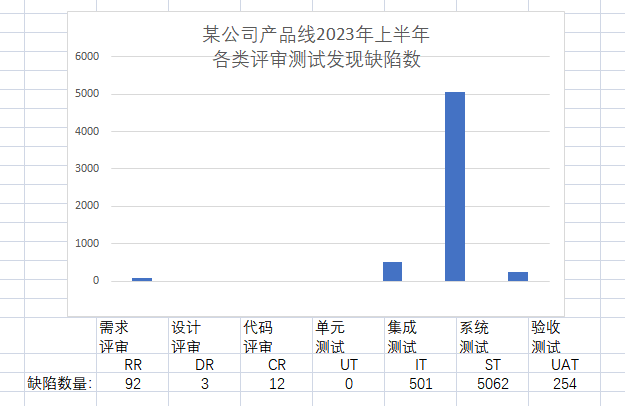
\includegraphics[width=6cm]{微信截图_20231023085822.png}

%由于测试与缺陷修复而造成返工的总工作量,在整个开发项目中占比很高\\

但很多开发人员误以为编码是项目主要工作,忽视了大量因质量问题引起返工,所以只有当管理层了解了尽早发现并排除缺陷是很好的改进方向,并引起重视,公司才有机会改进。

\framebox{%
\begin{minipage}[t]{0.97\columnwidth}\raggedright
有些偏业务的领导可能会质疑,客户不一定关注缺陷密度,只要达到可接受的水平就可以了。

我解释“在软件开发中,减少后期测试才发现的缺陷,不仅仅能提升产品质量,更重要的是能降低研发的总工作量,所以最终能帮助公司省钱。”(详见附件“公司高层不一定关注质量”)
\strut
\end{minipage}}

\hypertarget{ux5206ux6790ux7f3aux9677ux6392ux9664ux7387ux964dux4f4eux8d28ux91cfux6210ux672c}{%
\subsection{分析缺陷排除率降低质量成本}\label{ux5206ux6790ux7f3aux9677ux6392ux9664ux7387ux964dux4f4eux8d28ux91cfux6210ux672c}}

质量大师裘兰博士 (Dr JURAN) 强调,过程改进应从认同必须改善质量(Proof of the Need)开始。前面第8章的案例说明了如后期暴露的缺陷能预先在之前评审或单元测试发现便能大量减少项目成本,主要是质量成本(详见附件)。\\

%\href{文件:jalote_emm_7.1_1.0.png}{500px}

%\includegraphics[width=6cm]{jalote_emm_71_10.png}

但应如何开始? 

“应先考虑如何能收集到修复缺陷相关工时数据?因没有度量,便无法谈改进。一般团队(如果用系统管理缺陷)只有缺陷统计数据,缺少缺陷返工工作量,测试工作量数据。”\\

没有缺陷返工工作量数据,开发团队便不会觉得需要前面预先发现缺陷并解决,会以为应先让测试人员找出问题,开发人员才修正。

下章会介绍如何分析迭代缺陷数据,计算缺陷排除率,并举例说明,若提高前面评审、自测缺陷排除率能降低多少返工工作量。


\hypertarget{ux7ed3ux675fux8bed}{%
\subsection{结束语}\label{ux7ed3ux675fux8bed}}

可以让团队迭代回顾时收集并分析数据,解决公司级统一收集数据的困难。除了收集开发数据,也需要收集客户反馈数据,才全面,但也应每轮交付收集,才能及时分析数据。缺陷返工占软件开发工作量最多,缺陷越后发现,返工量越大。可以分析缺陷排除率,加强前面的代码扫描与评审,单元测试等,尽早发现并解决缺陷,不仅仅提供产品质量,也降低质量成本,提升团队生产率。

\begin{itemize}
\tightlist
\item
  为了确保质量应该用精益的概念。每一小步确认限制级,确保达标。然后与客户确认,而不是先定一个总体的几个月计划。按总计划监控任务是否延误?因为后者会把团队的关注点都放到按时交付去,无法确保最终的产品达到高质量要求。
\item
  迭代回顾让团队可以每走一小步,回顾有那些不足,分析根因,下一步做改善。如果要从``救火''的管理思路变成基于根本原因找出预防措施的思路,就需要管理者`放手',让团队自己收集数据,自己分析与制定纠正措施。
\item
  收集数据很重要:

  \begin{itemize}
  \tightlist
  \item
    收集数据应与迭代冲刺同步,除了收集团队内数据,也要收集客户的意见,才能全面看清问题
  \item
    如果把数据关连到绩效,很可能会`污染'数据,影响数据的正确性
  \item
    数据有显著变化时,便应更新基线,不要等到年底才更新
  \end{itemize}
\end{itemize}

下一章,我们探索如何策划好迭代回顾与相关培训,让团队回顾后能提升质量和生产率。

\hypertarget{ux9644ux4ef6}{%
\section{附件}\label{ux9644ux4ef6}}

\hypertarget{ux8d28ux91cfux6210ux672c-coq-cost-of-quality}{%
\subsection{质量成本 COQ (Cost of
Quality)}\label{ux8d28ux91cfux6210ux672c-coq-cost-of-quality}}

质量成本由三部分组成:

\begin{enumerate}
\tightlist
\item
  失效(Failure)成本\\
  把缺陷修复好的成本,包括在客户现场被发现的缺陷。
\item
  评测(Appraisal)成本\\
  包括各类测试,如系统测试,集成测试,单元测试等,所花的工时
\item
  预防(Prevention)成本\\
  包括技术评审 (注:有些人把评审归为评测成本,这里按 Mr.Juran
  定义,归属于预防成本)
\end{enumerate}

如变通理解以上COQ定义,``如何通过提高评审效率来降低质量成本``便可对应COQ各部分:\\
失效(Failure)成本:原本所有与缺陷相关的成本\\
评测(Appraisal)成本:增加测试前的静态扫描、评审,减少失效(Failure)成本,使总COQ下降\\
预防(Prevention)成本:减小缺陷的产生,例如用原型做好需求,进一步使总COQ下降\\

\hypertarget{ux516cux53f8ux9ad8ux5c42ux4e0dux4e00ux5b9aux5173ux6ce8ux8d28ux91cf}{%
\subsection{公司高层不一定关注质量}\label{ux516cux53f8ux9ad8ux5c42ux4e0dux4e00ux5b9aux5173ux6ce8ux8d28ux91cf}}

\framebox{%
\begin{minipage}[t]{0.97\columnwidth}\raggedright
{问}:在传统 IT的
公司,无论是 缺陷(Bug)
率还是其他质量指标对业务的影响的相关性都不容易度量,只有重大事件才会让公司在客户面前失去信任,所以高层不会真正的重视质量。\\
{答}:理解,但软件BUG的暴露越往后,返工的工作量就越高,而且是几何级数的增加(例如在单元测试或评审发现都可以1人时内解决;系统测试通常要花起码20人时,客户使用后才发现便更高)。但在很多IT公司,大部分缺陷都是在系统测试、甚至到验收测试才发现。如果能把软件缺陷的发现前移,把通过系统测试、验收测试发现的缺陷减半,便可以大量降低质量成本,提升开发生产率。所以我建议利用缺陷数估算返工的工作量来引起老板重视。(而不是仅仅说降低缺陷率)\\
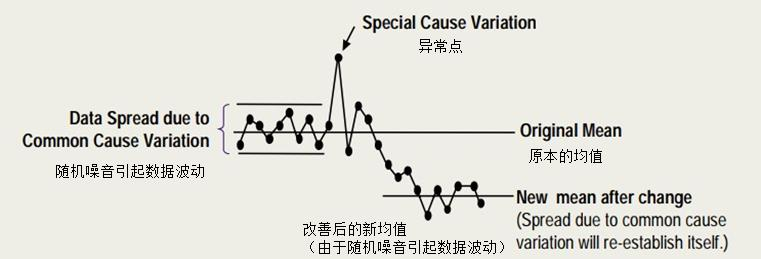
\includegraphics[width=6cm]{MGR_f11.jpg}
\strut
\end{minipage}}

\hypertarget{ux5f00ux53d1ux9879ux76eeux5de5ux4f5cux91cfux6210ux672cux5206ux5e03}{%
\subsection{开发项目工作量(成本)分布}\label{ux5f00ux53d1ux9879ux76eeux5de5ux4f5cux91cfux6210ux672cux5206ux5e03}}

参考Capers JONES先生 2012 的例子,汇总成以下比例:

%\url{文件:AR1成本占比.jpg}
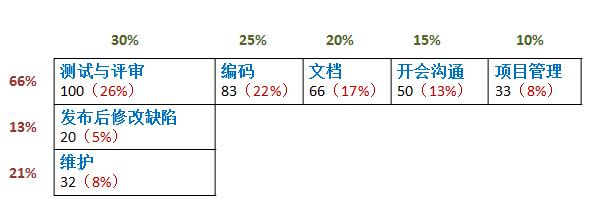
\includegraphics[width=6cm]{AR1成本占比.jpg}

测试与评审一般占开发工作量的30\%,测试与评审一般占总质量成本(包括发布后维护与改缺陷工作)的66\%,把所有工作量都加起来,测试与评审还是占最大(26\%)
, 编码第二 (22\%)。

\framebox{%
\begin{minipage}[t]{0.97\columnwidth}\raggedright
注意:测试与评审包括所有与缺陷相关的成本,包括单元测试、静态扫描、评审与相关的缺陷修正,
而编码只包括设计与编写代码部分。 例如有些人会觉得比例应该是
开发30\%,测试和bug修改25\%,需求和设计20\%,项目管理和沟通20\%,文档5\%。

但如果按上面的定义,开发部分很可能已包括单元测试、静态扫描与改正缺陷工作,
如把这些都归到测试评审里会变回类似上图的比例。\strut
\end{minipage}}


